%%%%%%%%%%%%%%%%%%%%%%%%%%%%%%%%%%%%%%%%%
% Stylish Title Page
% LaTeX Template
% Version 2.0 (22/7/17)
%
% This template was downloaded from:
% http://www.LaTeXTemplates.com
%
% Original author:
% Peter Wilson (herries.press@earthlink.net) with modifications by:
% Vel (vel@latextemplates.com)
%
% License:
% CC BY-NC-SA 3.0 (http://creativecommons.org/licenses/by-nc-sa/3.0/)
% 
% This template can be used in one of two ways:
%
% 1) Content can be added at the end of this file just before the \end{document}
% to use this title page as the starting point for your document.
%
% 2) Alternatively, if you already have a document which you wish to add this
% title page to, copy everything between the \begin{document} and
% \end{document} and paste it where you would like the title page in your
% document. You will then need to insert the packages and document 
% configurations into your document carefully making sure you are not loading
% the same package twice and that there are no clashes.
%
%%%%%%%%%%%%%%%%%%%%%%%%%%%%%%%%%%%%%%%%%

%----------------------------------------------------------------------------------------
%	PACKAGES AND OTHER DOCUMENT CONFIGURATIONS
%----------------------------------------------------------------------------------------

\documentclass[a4paper, 11pt, oneside]{book} % A4 paper size, default 11pt font size and oneside for equal margins

\usepackage[svgnames]{xcolor} % Required for colour specification

\usepackage{graphicx} % Required for box manipulation
\usepackage{float}

\newcommand*{\plogo}{\fbox{$\mathcal{PL}$}} % Generic dummy publisher logo

\usepackage[utf8]{inputenc} % Required for inputting international characters
\usepackage[T1]{fontenc} % Output font encoding for international characters
\usepackage{PTSerif} % Use the Paratype Serif font

\usepackage[utf8]{inputenc}
\usepackage[utf8]{inputenc} % set input encoding to utf8
\usepackage{xcolor}
\usepackage{booktabs}
\usepackage{longtable}
\usepackage{hyperref}
\usepackage{graphicx}
\usepackage{float}
\usepackage{titling,lipsum}
\usepackage{geometry}
\usepackage{miama}
\usepackage{addfont}
\usepackage[T1]{fontenc}
\usepackage[]{moresize}


\begin{document} 

\addfont{OT1}{necker}{\necker}
%----------------------------------------------------------------------------------------
%	TITLE PAGE
%----------------------------------------------------------------------------------------

\begin{titlepage} % Suppresses headers and footers on the title page

	\centering % Centre all text
	
	%------------------------------------------------
	%	Title and subtitle
	%------------------------------------------------
	
	\setlength{\unitlength}{0.6\textwidth} % Set the width of the curly brackets above and below the titles
	
	{\color{LightGoldenrod}\resizebox*{\unitlength}{\baselineskip}{\rotatebox{90}{$\}$}}}\\[\baselineskip] % Top curly bracket
	
	\textcolor{Sienna}{\textit{\Huge Laureate Award for Excellence in Robotics Engineering 2018}}\\[\baselineskip] % Title
	
	{\color{RosyBrown}\Large Universidad del Valle de México}\\ % Subtitle or further description
    {\color{RosyBrown}\Large (Campus Monterrey)}
	
	{\color{LightGoldenrod}\resizebox*{\unitlength}{\baselineskip}{\rotatebox{-90}{$\}$}}} % Bottom curly bracket
	
	\begin{figure}[H]
	    \label{fig:ide}
	    \centering
        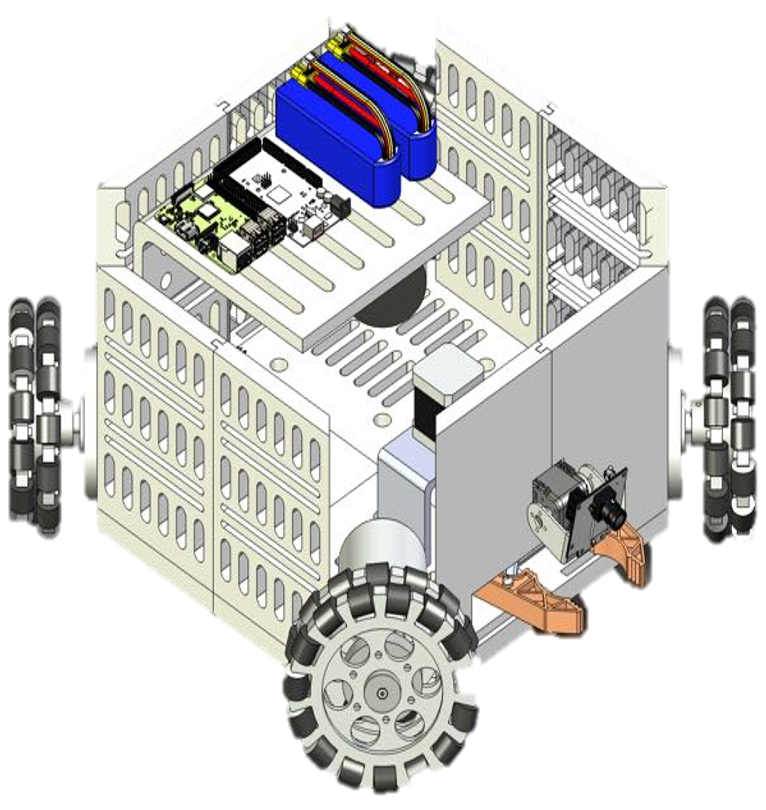
\includegraphics[scale = 0.8]{ourRobot3}
	    %\caption{Integrated Development Environment (IDE)}
    \end{figure}
	\vfill % Whitespace between the title and the author name
	
	%------------------------------------------------
	%	Author
	%------------------------------------------------
	
	\textcolor{Sienna}{\necker \HUGE <<Equipo Atl>>}\\ % Author name
	\vfill % Whitespace between the author name and the publisher logo
	
	%------------------------------------------------
	%	Publisher
	%------------------------------------------------
	
	%\plogo\\[0.5\baselineskip] % Publisher logo
	
	%The Publisher % Publisher name
	{\color{RosyBrown}\fmmfamily \Huge 18 de mayo de 2018}

\end{titlepage}

%----------------------------------------------------------------------------------------

\end{document}
